\chapter{REVIEW OF RELATED LITERATURE}

\section{Software Defined Networking}
Software-defined networking (SDN, also refers to \textit{software defined networks}) is a networking architecture that arose due to the need for a centralized control, programmability and automation in a network \cite{open_networking_foundation_software-defined_2013}. In traditional networks, fulfilling this requirement meant specific control of different forwarding devices in the network, each with its own control plane (deciding how to handle network traffic) and forwarding plane (forwarding traffic according to the decisions made by the control plane) \cite{kreutz_software-defined_2015}. To solve this, SDN separates the forwarding plane from the control plane, and introduces the concept of a logically centralized \textit{controller} \cite{open_networking_foundation_software-defined_2013}. In this model, network devices simply become forwarding devices which receive instructions from the controller on how it treats different types of network traffic. Network applications such as traffic engineering, monitoring and security such as firewalls can interact with the controller, instead of the network itself \cite{kreutz_software-defined_2015}.

\section{OpenFlow and OpenFlow-based SDN Controllers}
OpenFlow is a protocol that allows controllers to communicate with forwarding devices in a standardized way, first proposed by McKeown et. al. \cite{mckeown_openflow_2008}. In OpenFlow, instructions on incoming traffic is \textit{flow-based}. A \textit{flow} is a sequence of packets from a source to a destination, which receive the same treatment at forwarding devices. The controller controls all of these flows; therefore, the controller an is an abstraction of the underlying network. OpenFlow consists of message types that control the behavior of forwarding devices (in this case, \textit{OpenFlow switches}), and message types that where forwarding devices tell the controller about the its own status \cite{open_networking_foundation_openflow_2009}. The \textit{Secure channel} connects the controller to OpenFlow switches, and all OpenFlow messages are sent through this channel. When an OpenFlow switch encounters a packet, it sends a \textsc{Packet-In} message to the controller. The controller then instructs the switch that sent the message to perform some \textit{action} on the packet. This action can be dropping a packet, forwarding a packet to a port, or making modifications to the data before forwarding the packet. Additionally, the controller can send a \textit{Flow-Mod} instruction that allows the OpenFlow switch to remember in its \textit{Flow Table} the action/s taken on packets that \textit{match} certain characteristics \cite{open_networking_foundation_openflow_2009}. In summary, the role of the OpenFlow controller is to instruct the forwarding devices on how to treat incoming network traffic.

The controller is implemented as \textit{software} that manages the network devices. Examples of OpenFlow controllers include  POX, OpenDaylight, Floodlight and Ryu \cite{salman_sdn_2016}. POX was used in Pena and Yu \cite{pena_development_2014} to successfully implement a distributed firewall, with testing done in Mininet, a testbed for simulating realistic networks in a single machine \cite{noauthor_mininet_nodate}. This thesis used Ryu because it is relatively well documented among the Python-based controllers \cite{salman_sdn_2016}. Ryu is an open source framework that provides basic controller functionality for SDNs. It facilitates an SDN application development, and supports a wide range of the OpenFlow specifications, making it appropriate for the development of network applications \cite{kubo_ryu_2014}. 


\section{Quality of Service}
Quality of Service (QoS) is a set of technologies aimed at providing a certain level of guarantee to resource intensive or performance sensitive traffic flow from important applications such as VoIP, video conferencing, and online gaming. Metrics used to assess QoS include delay, bandwidth, jitter, and packet loss \cite{karakus_quality_2017}. The two largest QoS architectures in traditional networks are IntServ and DiffServ. IntServ works by the individual routers reserving a portion of resources with the Resource Reservation Protocol in order to provide quantifiable QoS per flow \cite{braden_rfc1633_1994}. While this allows for exact control of QoS guarantees, it requires that all routers support the protocol, which means that it does not scale well. DiffServ works with aggregated classes of IP packets based on the Differentiated Service Code Point (DSCP) field to change the Per-Hop Behavior (PHB), which describes how each packet is treated per forwarding device, usually relative to other PHBs \cite{blake_rfc2475_1998}. While DiffServ allows for better scalability and simpler configuration, it leaves control policy as a separate issue, therefore it is harder to have fine-grained control of traffic \cite{zhao_internet_2000}.


\section{QoS Provisioning and Management in SDN}
The previous examples of IntServ and DiffServ show that configuring disparate devices is not suitable to meet the constantly changing demands of QoS. Software-defined networking alleviates this problem by providing a logically central point of control that can abstract the network into a consistent API that network applications can work with \cite{kreutz_software-defined_2015}. Because of this, QoS Provisioning with Software-defined networking has been an important topic of research in the last decade, with many attempts to simulate various conditions and QoS provisioning methods over different platforms and environments.

QoS Routing is a basic problem of QoS Provisioning where the paths that packets take need to satisfy a wide range of QoS constraints \cite{zheng_wang_quality--service_1996}. SDN enables for more sophisticated methods of routing based on QoS parameters, instead of defaulting to the shortest path routing. Kuipers and Van Mieghem \cite{goos_qos_2001} provided an exact algorithm that guarantees to find a path that satisfies QoS constraints, if it exists, and tested the algorithms on random graphs. Kaiming and Liu \cite{kaiming_liu_novel_2016} introduced a new algorithm to find QoS routing paths in SDN based wireless mesh networks. They used heuristics to solve a NP-Hard problem by dynamically updating weight based on delay and packet loss rate and tested it on Mininet-Wifi with 10 routers and 8 clients.

SDN also enables queue management through the use of OF-CONFIG \cite{bansal_-config_2014} and OVSDB (OpenVSwitch Database) \cite{pfaff_rfc_2013} protocols. Queues are used to shape traffic and limit their bandwidth usage, thereby dividing the resources of the network among different types of traffic. Yan, Zhang, Shuai, Liu and Guo used a combination of multi-path routing and queue separation for different types of traffic to achieve better performance in throughput and resilience \cite{yan_hiqos_2015}. They use Mininet and Floodlight to simulate a relatively simple 5-node, topology with 11 clients and 2 servers. Sudiharto et. al. used a VoIP network setting to compare class-based queuing and priority queuing \cite{sudiharto_comparative_2015}. They used the NS-2 simulator to simulate a topology with 3 servers and 3 clients to find that class-based queuing was the more effective method. Ishimori, Farias, Cerqueira and Abelem used the Stochastic Fairness Queuing technique instead of the First-in-first-out technique to improve Quality of Experience \cite{ishimori_control_2013}. However, the test were limited to the single-switch topology and the linear topology. Chato and Yu investigated different class-based queuing (CBQ) techniques enforced on the core and on the leaves, but experiments were limited to a 3-switch tree topology \cite{chato_exploration_2016}.

\section{QoS and Network Topology}
Different network topologies have different applications, strengths and weaknesses. Mesh networks, for example, are used to maintain reliable and self-healing connections throughout the network \cite{chawla_fault_2015}. Ring networks are used mostly in local area networks where connection is maintained even if one node fails, and since each node has two neighbors, routing is simple. The tree topology is suitable for large geographical areas and thus can be implemented for large-scale networks such as Metropolitan Area Networks \cite{gerla_tree_1988}. Hypercube networks are commonly used in parallel computing applications for inter-networking multiple processors each with their own memory modules \cite{yan_fundamentals_2009}.

While QoS provisioning research as shown in Section 2.2 focused on QoS provisioning, they did not test these techniques in different topologies, especially live networks. However, some work has been done in evaluating QoS techniques and characteristics in different topologies. Guck, Bemten, Reisslein, and Kellerer \cite{guck_unicast_2018} tested many QoS Routing techniques in ring topologies and grid topologies with different sizes. They considered shortest-path and constrained shortest path algorithms for routing, and concluded that different routing algorithms are the best for different topology configurations. Laassiri \cite{laassiri_evaluation_2017} evaluated packet loss, gigue, latency, and end-to-end delay in star, ring, tree, and hierarchical topologies in an SDN network. Regencia and Yu was able to generalize the simple three-node tree topology in the aforementioned study from Chato and Yu to complete binary trees with up to 6 layers \cite{yang_introducing_2022}.

\section{Testing various QoS queuing techniques in SDN}
Community-driven open-source Network Operating System (NOS) software such as Floodlight, NOX, POX, and Ryu have been used in research for testing and simulation purposes. Karakus and Durresi lists research regarding QoS that used Mininet with NOS software to simulate their algorithms \cite{karakus_quality_2017}, such as the aforementioned study by Ishimori et. al. \cite{ishimori_control_2013} and the study by Yan et. al. \cite{yan_hiqos_2015}. Regencia and Yu \cite{yang_introducing_2022} presented a Mininet and Ryu based framework for simulating various QoS queue management algorithms based on the aforementioned previous work by Chato and Yu \cite{chato_exploration_2016}. Torres, Regencia and Yu \cite{kim_real_2021} extended the framework to simulate real-world traffic data from PCAP files. Network testing in these studies were conducted with various traffic generation tools such as Iperf (as in \cite{yan_hiqos_2015} and \cite{ishimori_control_2013}, or ApacheBench and VLC (as in \cite{chato_exploration_2016} and \cite{kim_real_2021}) to load the network with random or synthetic traffic.

\section{Current QoS Testing Framework from Regencia and Yu}
The framework by Regencia and Yu \cite{yang_introducing_2022} accepts custom QoS algorithms and custom parameters for a tree topology as input to a Ryu controller that implements a Level 2 learning switch. Clients, servers, and OpenFlow switches are simulated by Mininet. In the experiment using this framework, the clients configured by the framework continuously make HTTP and VLC video-on-demand requests as synthetic load to the network for 5 minutes. The simulator script launches the benchmarking software within the clients, and the Ryu SDN Controller serves as the controller to the simulated network. Figure \ref{fig:original_architecture} shows the architecture of this testing framework. This is the framework that this thesis intends to build and improve upon.

\begin{figure}[htbp!]
    \centering
    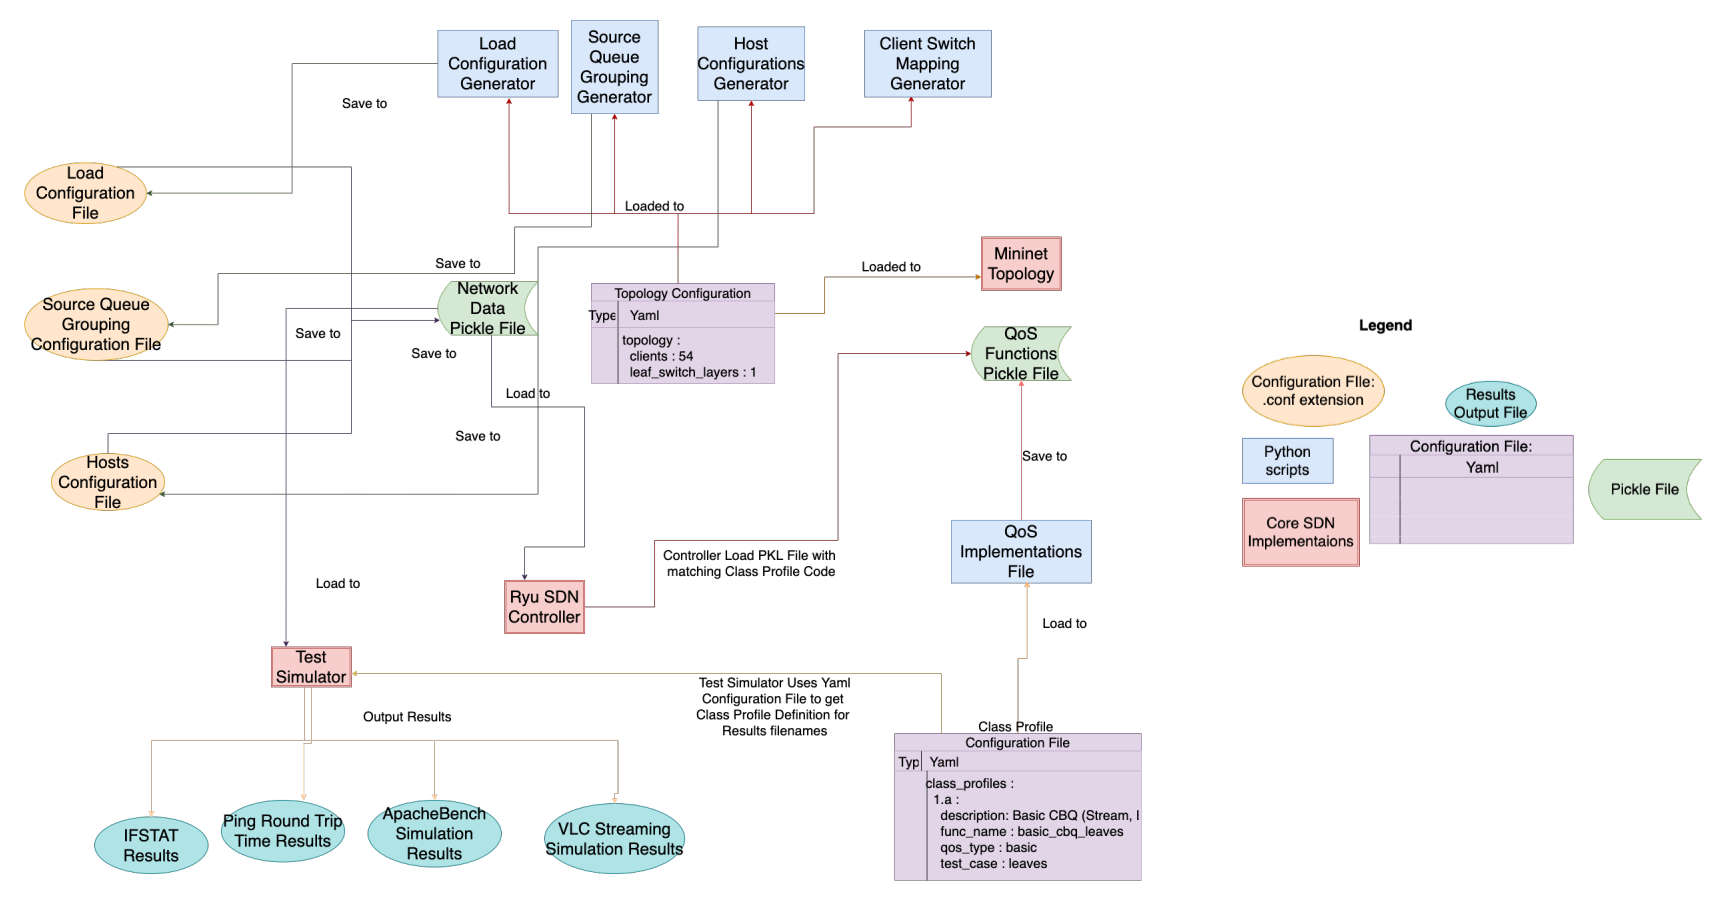
\includegraphics[width=\textwidth]{Figures/original_architecture.png}
    \caption{The architecture of the QoS Testing Framework}
    \label{fig:original_architecture}
\end{figure}

In this architecture, tests are configured with the \textit{Topology Configuration} file and the \textit{Class Profile Configuration File}. These contain the metadata of the network setup of the simulation, as well as the QoS queueing system to be used during the simulation. The metadata are loaded into scripts that generate Python-readable files for use in Mininet, Ryu, and a Python script for automating the execution of the test. The Python-readable files consists of the \textit{Load Configuration}, \textit{Source Queue Grouping Configuration}, and \textit{Hosts Configuration} files. Load Configuration is a list of clients and the requests that the client will make to the servers when running the tests. Source Queue Grouping Configuration contains the switches in the path from the client to a server. Hosts Configuration contains the basic information of each client and server, including the name, IP address, the connected switch, and protocols served.

\section{The Internet Topology Zoo in SDN Research}
The Internet Topology Zoo is a collection of network topologies traced from data provided by network operators around the world \cite{knight_internet_2011}. Some work was done with the Internet Topology Zoo (ITZ) as test data to simulate live networks. Mamushiane, Mwangama, and Lysko \cite{mamushiane_given_2018} test solutions to the placement of controllers in an SDN topology in ITZ data. Metter et. al. also used ITZ data to test the impact of network topology in the processing times of SDN controllers. \cite{metter_investigating_2015}. ITZ data is considered reliable because although it may not represent the networks exactly as running, it represents the network as the company providing the data intended to build. \cite{knight_internet_2011}

\section{Conclusion}
The reviewed literature shows that is important and necessary to test network algorithms in real-life situations, because real-life networks have complex topologies with multiple loops and many switches. There were no significant efforts to test QoS \textit{queuing techniques} in real-life topologies, which is a gap in the literature that this thesis aims to bridge. Since the framework from Regencia and Yu was intended to test different QoS algorithms in many situations, we can modify it to include ITZ data, which will allow for easier and better testing of simple and complex QoS techniques. This thesis will then bridge the aforementioned gap, as Guck et. al. \cite{guck_unicast_2018} was able to do with QoS \textit{routing} algorithms.

